\documentclass[UTF8]{article}
\usepackage{graphicx}
\usepackage{listings}
\usepackage{hyperref}
\graphicspath{ {Assignment3/} }


\begin{document}


\title{%
  CPS 1010- Collaborative Practical Project\\  
  \vspace{5mm}  
  \large Assignment 3-Issue Tracking and Continuous Integration}
\vspace{100mm}
\author{Ylenia Zammit, Darren Aquilina, Daniel Camilleri}
\date{28th November 2016} 
\maketitle

\newpage
\section{Team Information}
Our team consists of three members, Daniel Camilleri, Ylenia Zammit and Darren Aquilina.
\vspace{5mm}
\\
Darren Aquilina:
	18 years old. Very interested in software development as can be shown by previous experience in Java and newly acquired knowledge with the C programming language. 
	He brings excellent debugging skills to the team. His interests are physical activity and social gatherings.
\vspace{5mm}
\\
Ylenia Zammit:
	18 years old. Interested in web development with previous experience in JavaScript and HTML.
	She brings excellent motivation to the team as well as efficient problem solving techniques.
	Her interests include Karate and jogging.
\vspace{5mm}
\\
Daniel Camilleri: 19 years old. Intreseted in software and hardware development by building his own personal computer on the hardware side and learning basic Java programming and currently learning programming in C.
		  He brings excellent quality and unit testing. His interests are computer hardware and gaming.
\newpage
\section{Project Information}
Github Link : \url{https://github.com/danielsna/The-IT-Crew}
\vspace{5mm}
\\
The URL to Jenkins project : \url{https://jenkins-ict.research.um.edu.mt/job/The%20IT%20Crew/}
\newpage
\section{Screen shots of key parts of Jenkins configuration}
\begin{figure}[h]
  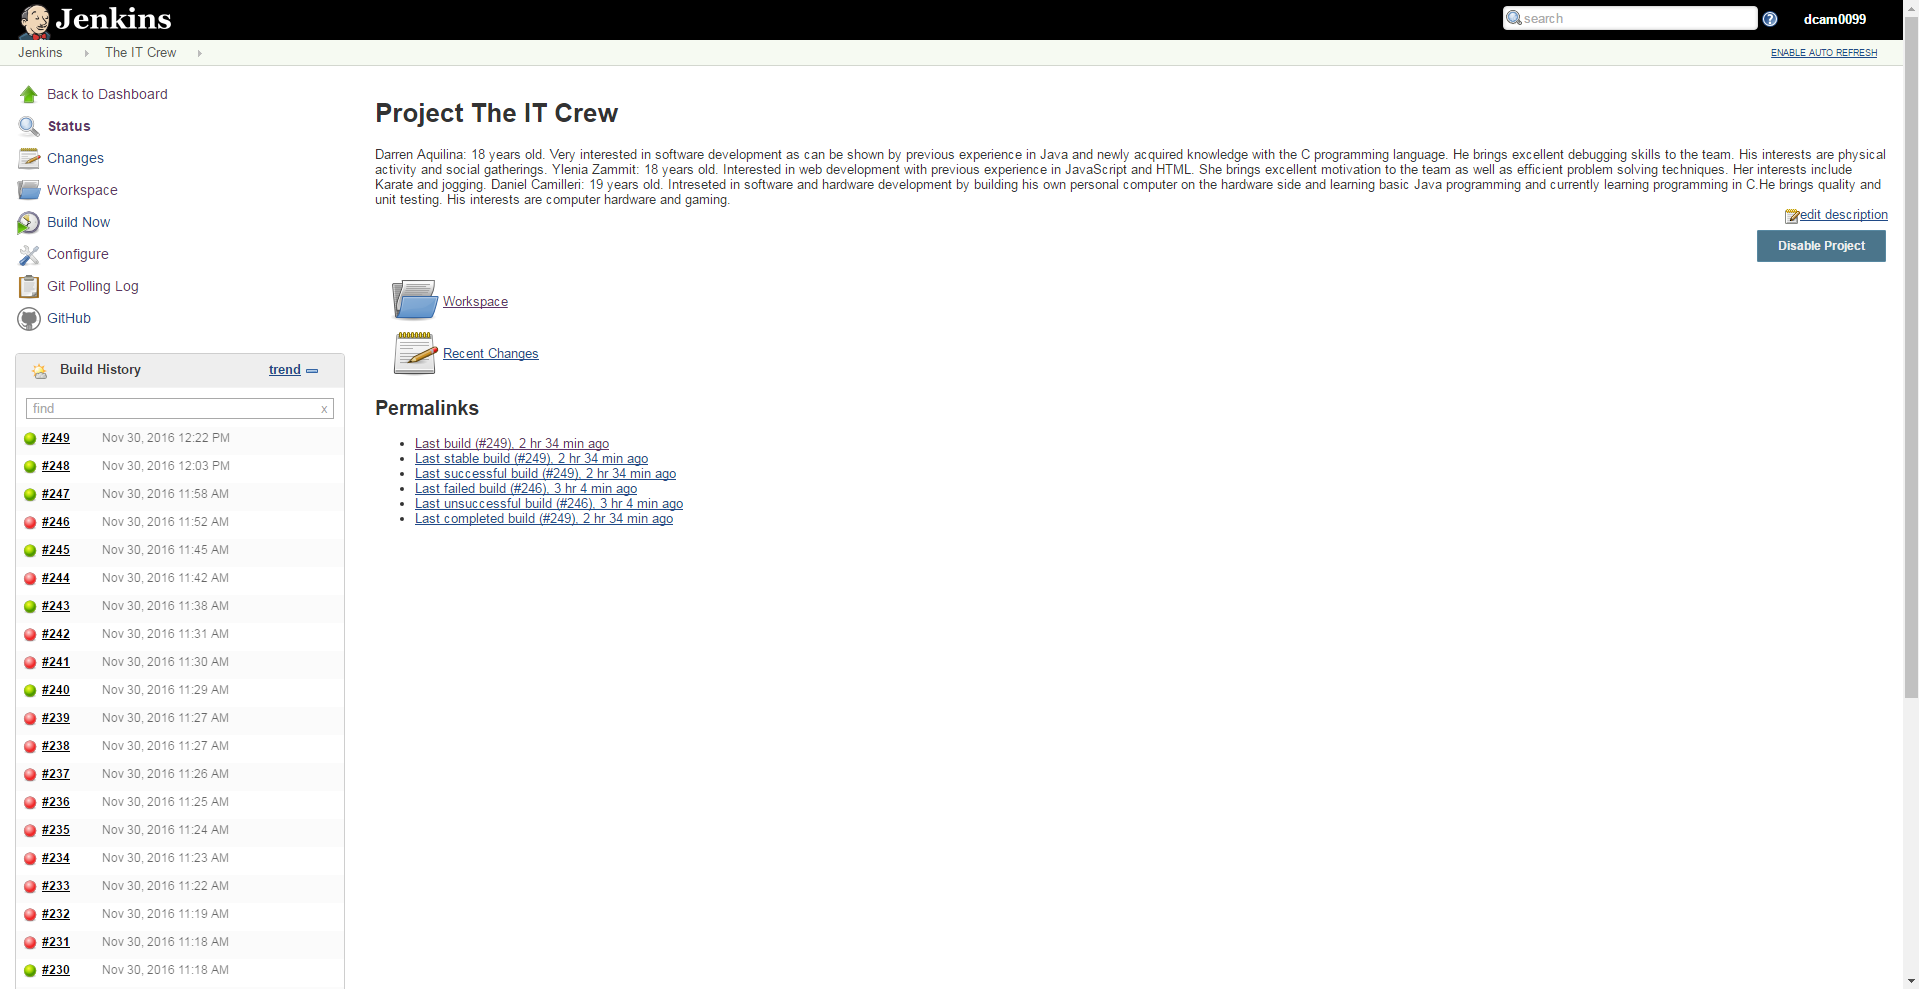
\includegraphics[width=\textwidth, height=\textheight,keepaspectratio]{JenkinsSetup0}
  \caption{Build output}
\end{figure}

\begin{figure}[h]
  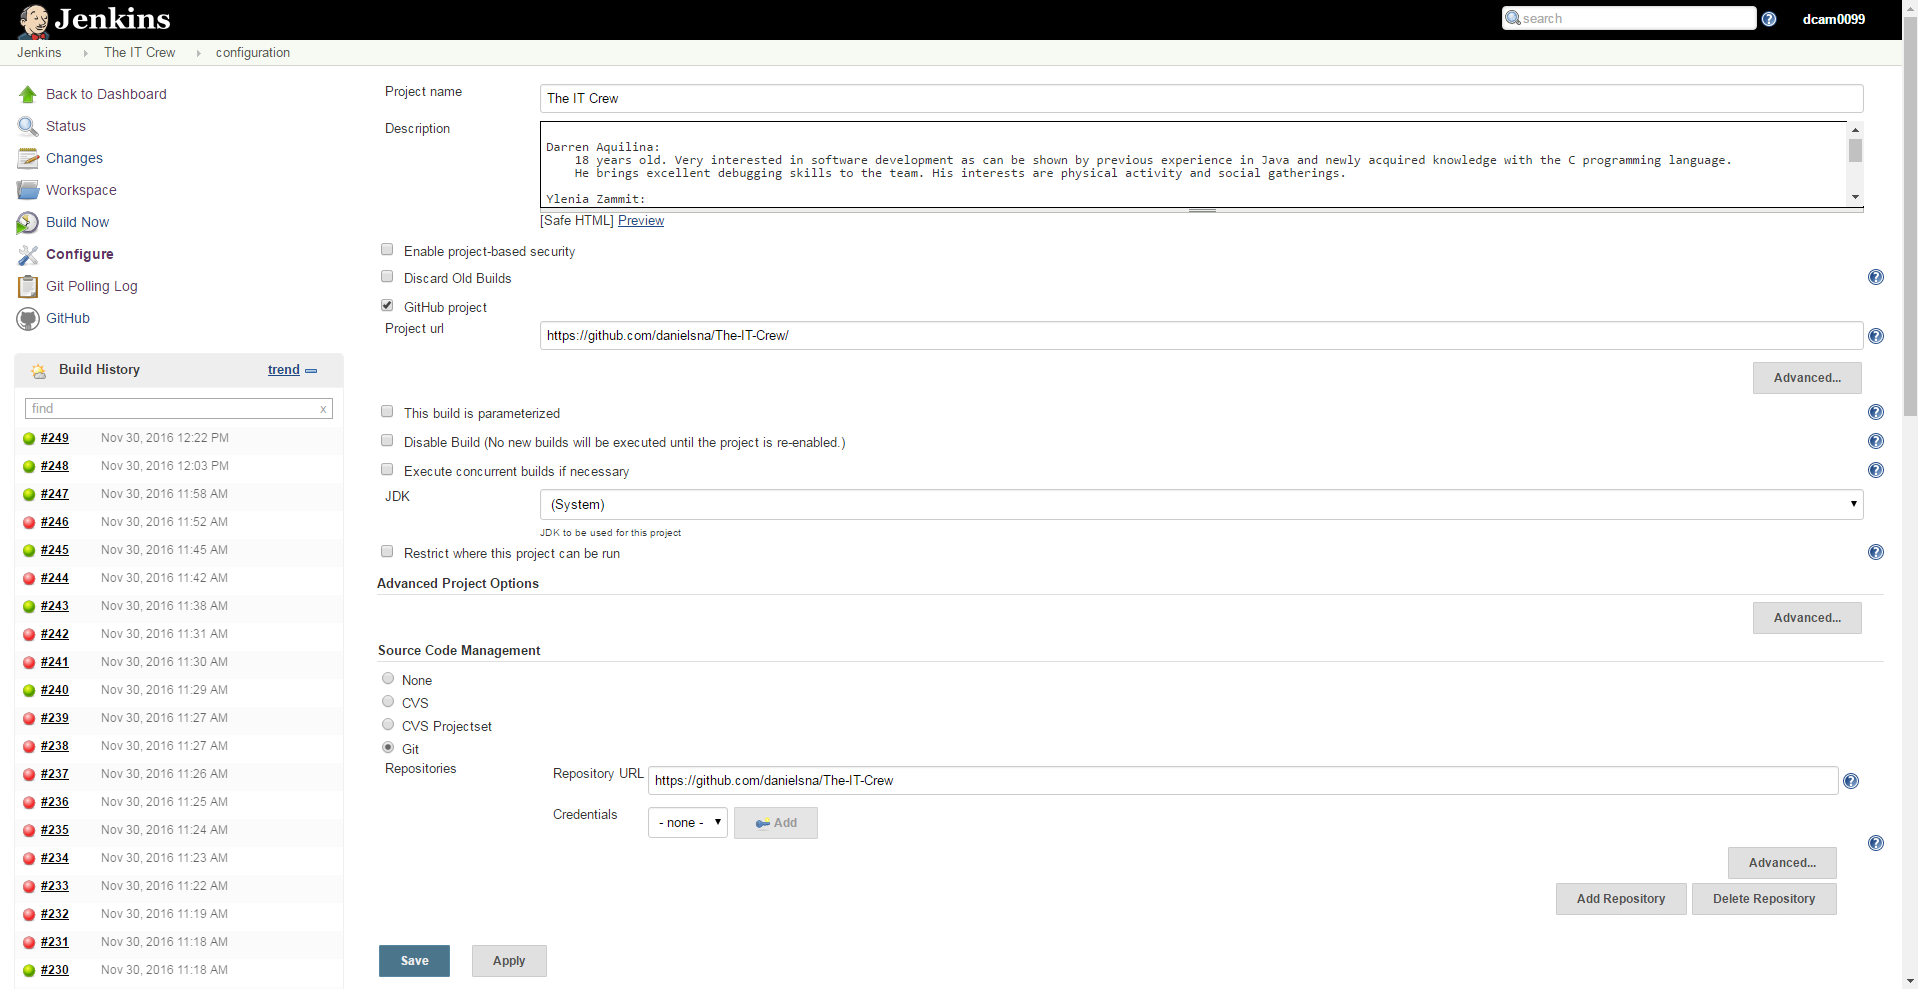
\includegraphics[width=\textwidth, height=\textheight,keepaspectratio]{JenkinsSetup1}
  \caption{Configuration Page: Part1}
\end{figure}

\newpage
\begin{figure}[h]
  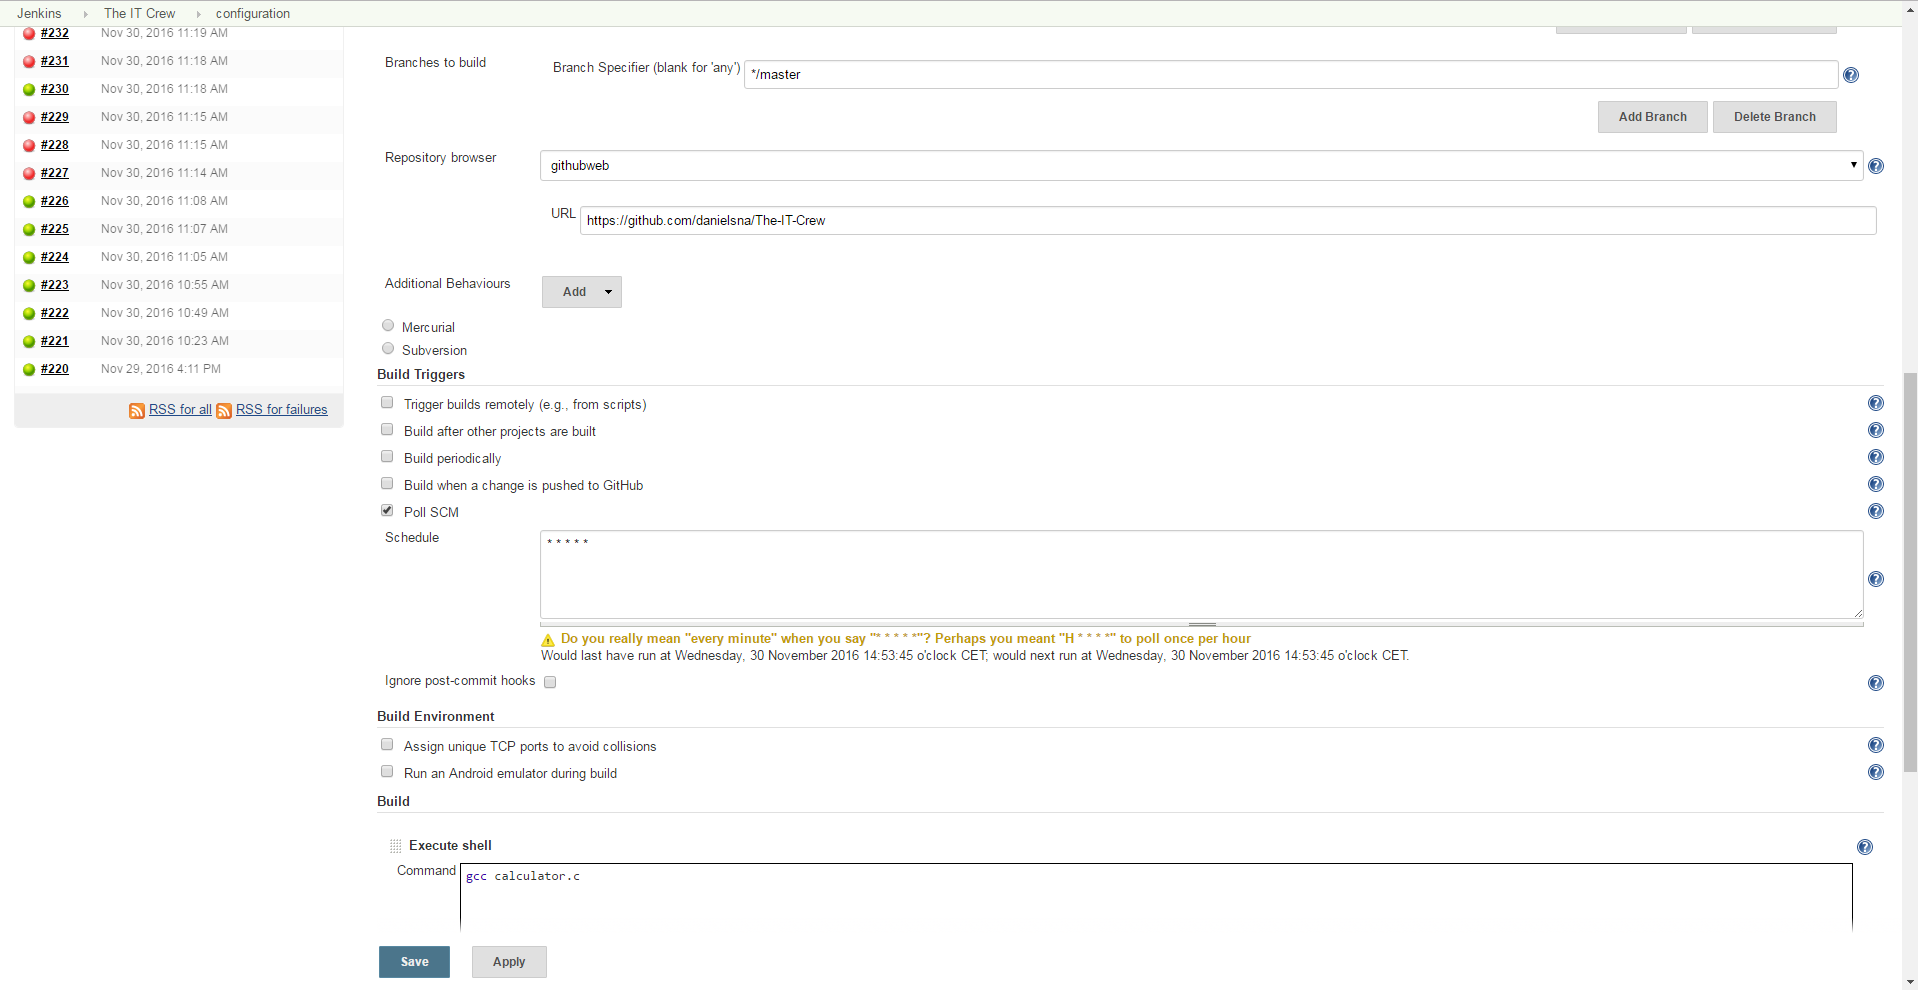
\includegraphics[width=\textwidth, height=\textheight,keepaspectratio]{JenkinsSetup2}
  \caption{Configuration Page: Part2}
\end{figure}

\begin{figure}[h]
  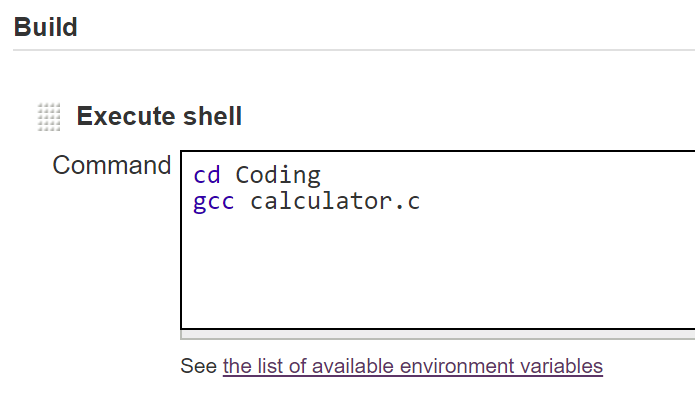
\includegraphics[width=\textwidth, height=\textheight,keepaspectratio]{ExecuteShell}
  \caption{Executing Shell Command}
\end{figure}

\newpage
\section{Screen shots of Generating and Fixing Errors}
\begin{figure}[h]
  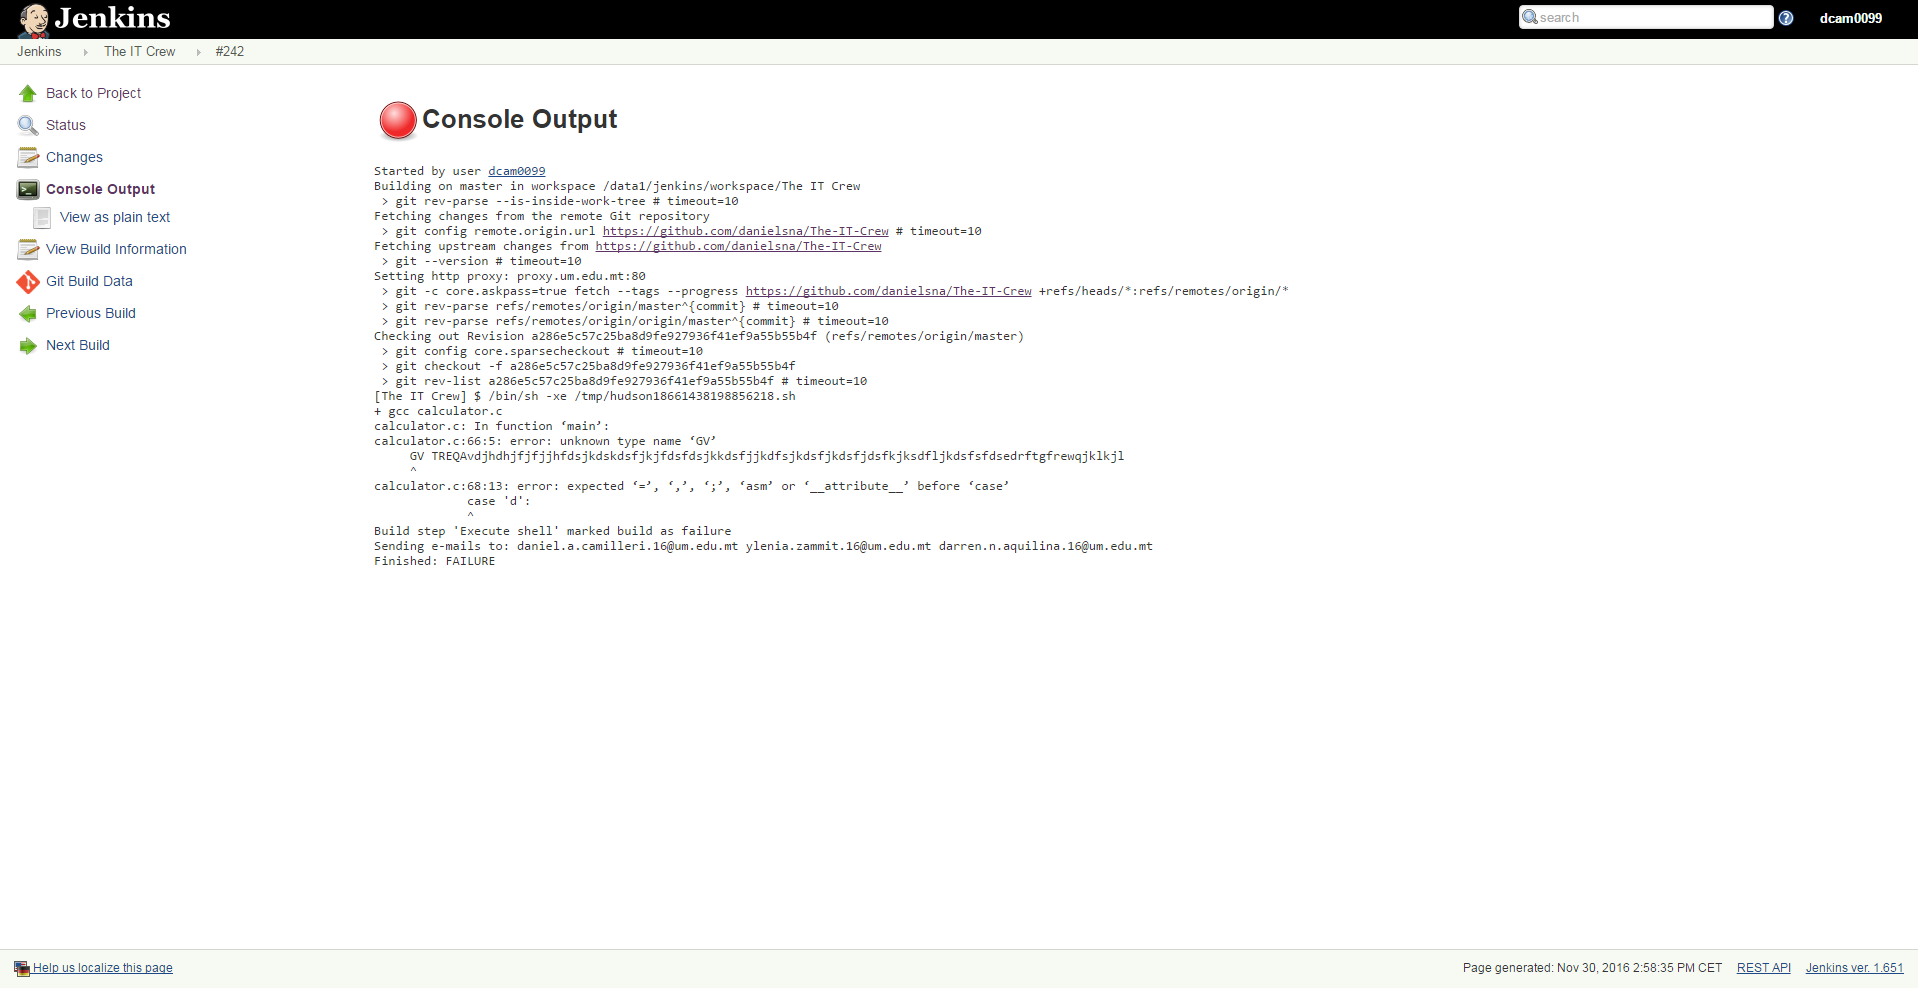
\includegraphics[width=\textwidth, height=\textheight,keepaspectratio]{Break1Daniel.PNG}
  \caption{Error generated by Daniel}
\end{figure}

\newpage
\begin{figure}[h]
  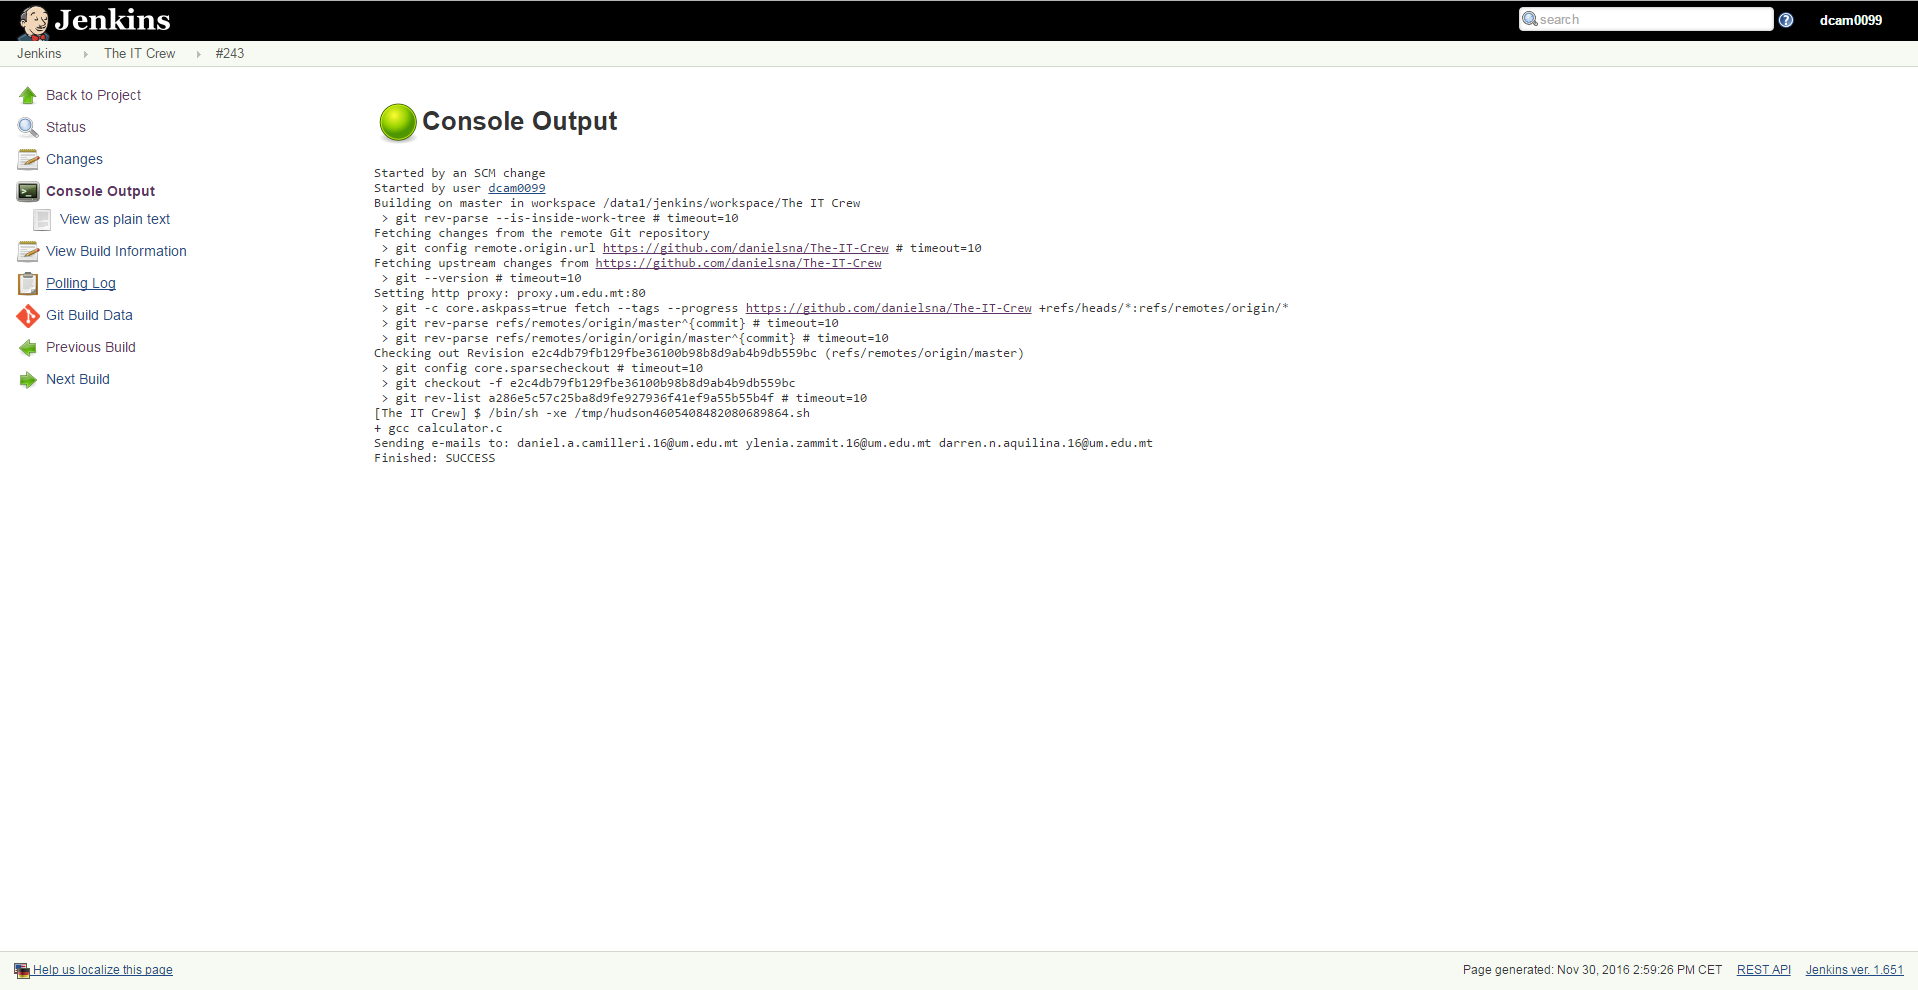
\includegraphics[width=\textwidth, height=\textheight,keepaspectratio]{BreakFix1Daniel.PNG}
  \caption{Error fixed by Daniel}
\end{figure}

\newpage
\begin{figure}[h]
  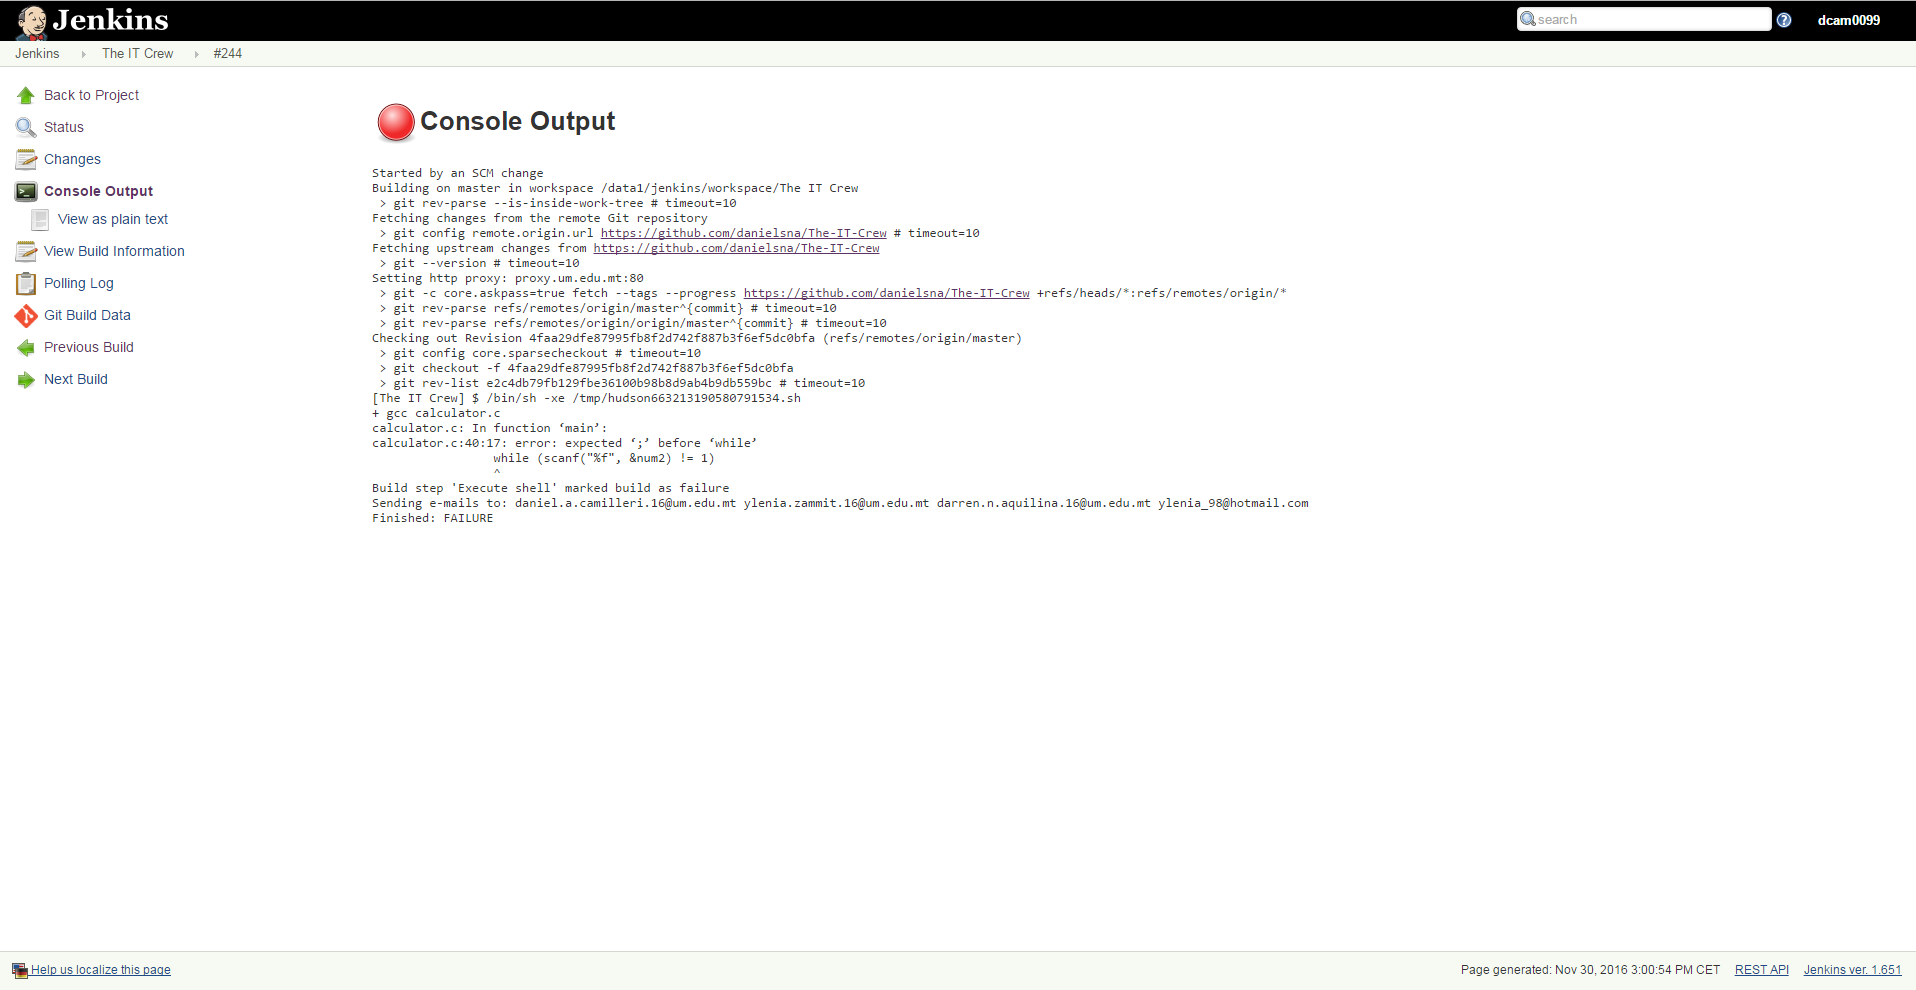
\includegraphics[width=\textwidth, height=\textheight,keepaspectratio]{Break2Ylenia.PNG}
  \caption{Error generated by Ylenia}
\end{figure}

\begin{figure}[h]
  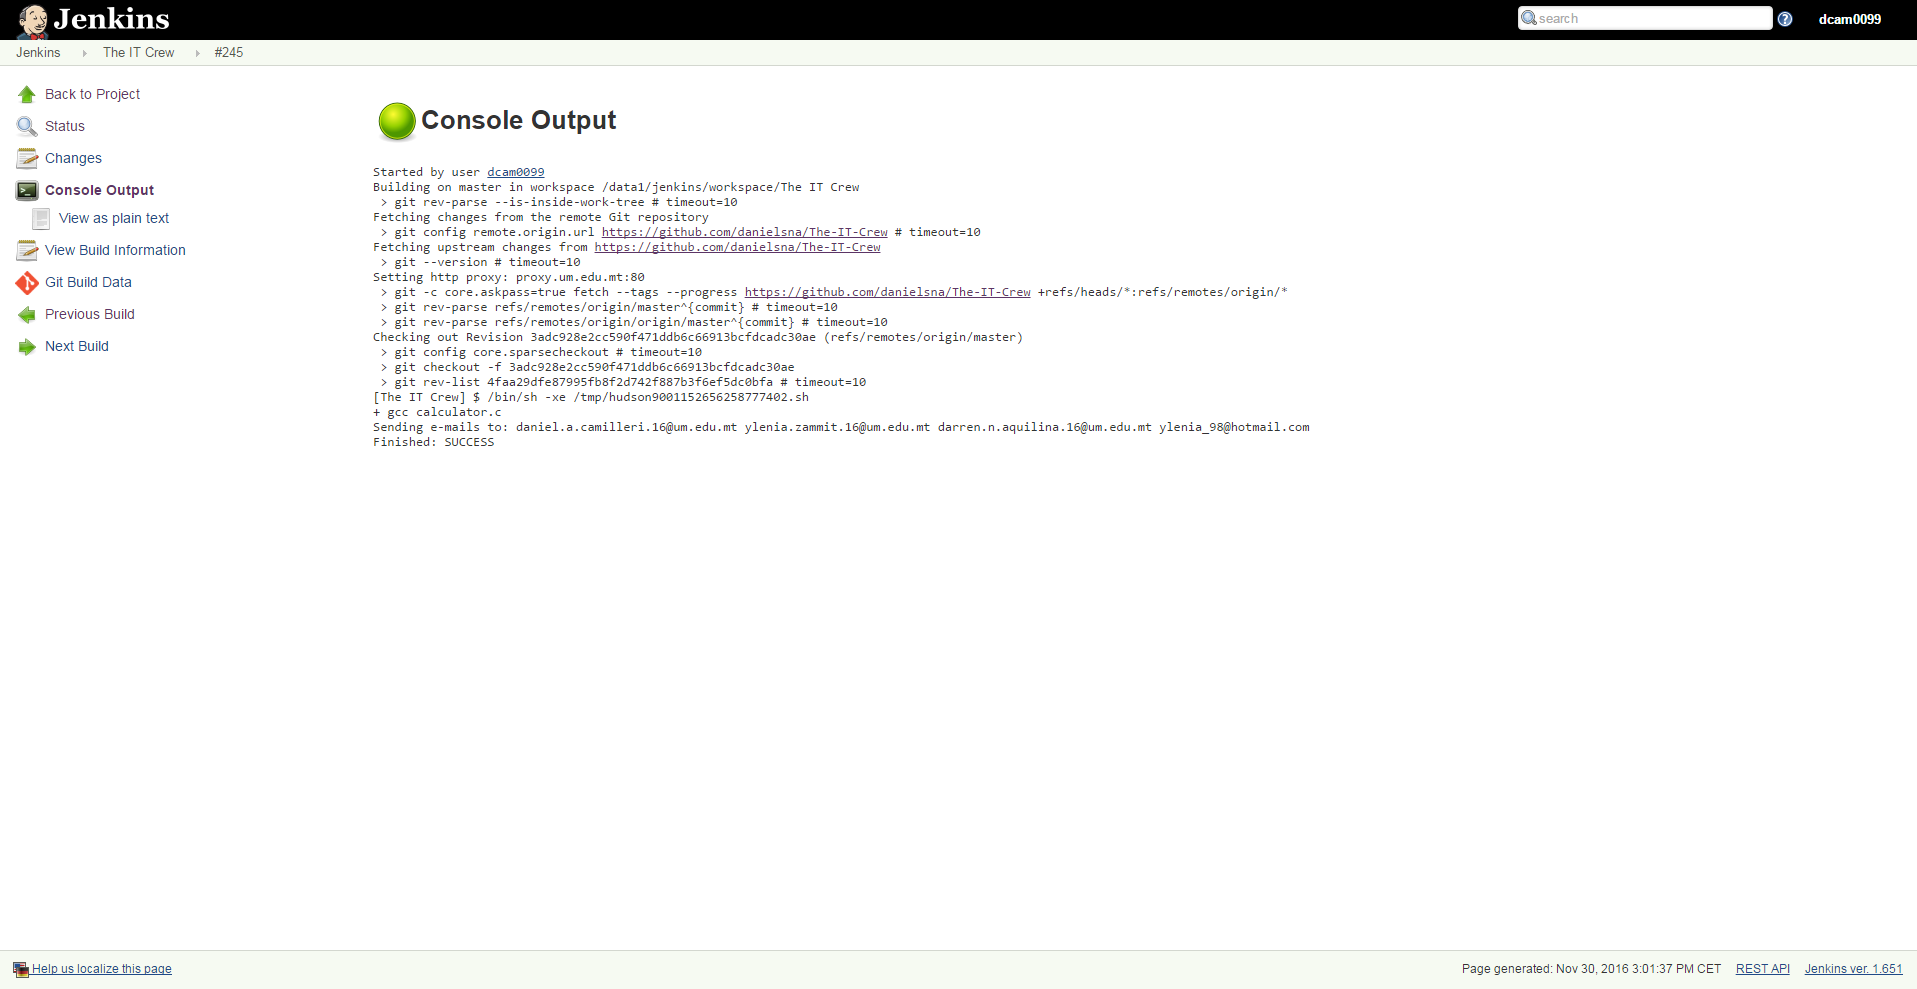
\includegraphics[width=\textwidth, height=\textheight,keepaspectratio]{Fix2Ylenia.PNG}
  \caption{Error fixed by Ylenia}
\end{figure}

\newpage
\begin{figure}[h]
  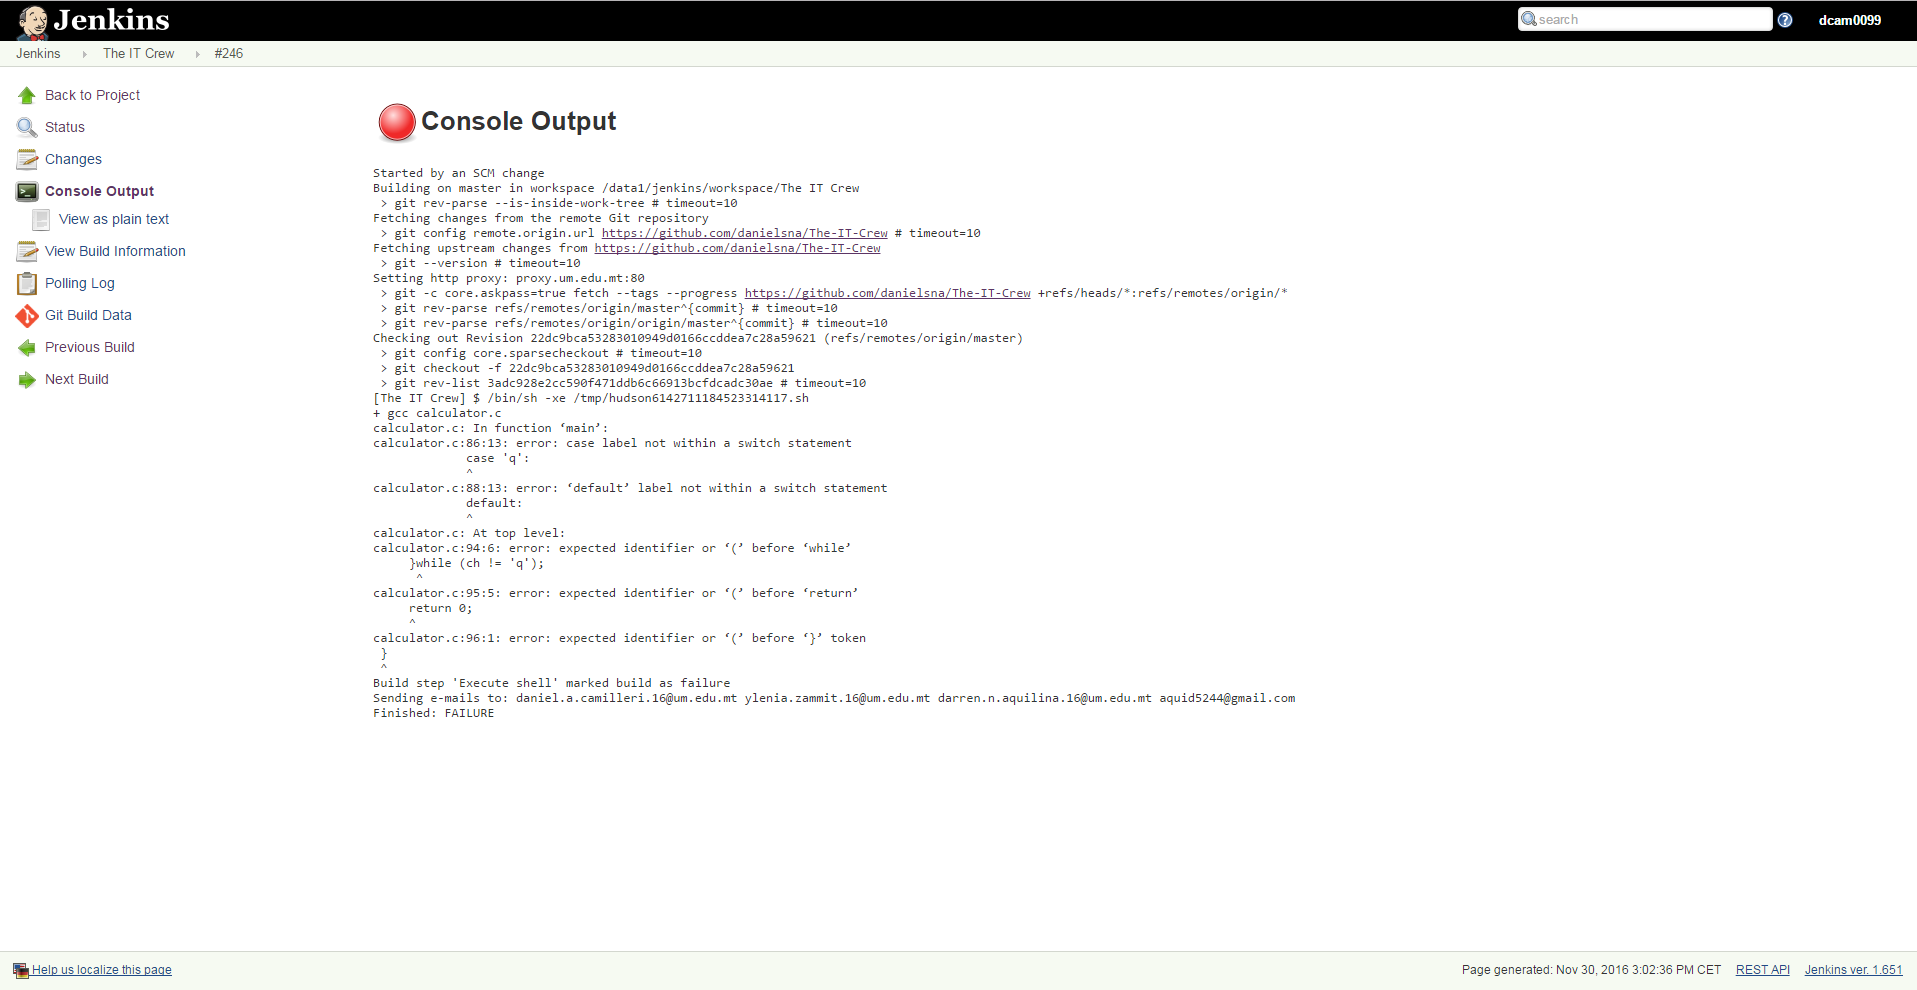
\includegraphics[width=\textwidth, height=\textheight,keepaspectratio]{Break3Darren.PNG}
  \caption{Error generated by Darren}
\end{figure}

\newpage
\begin{figure}[h]
  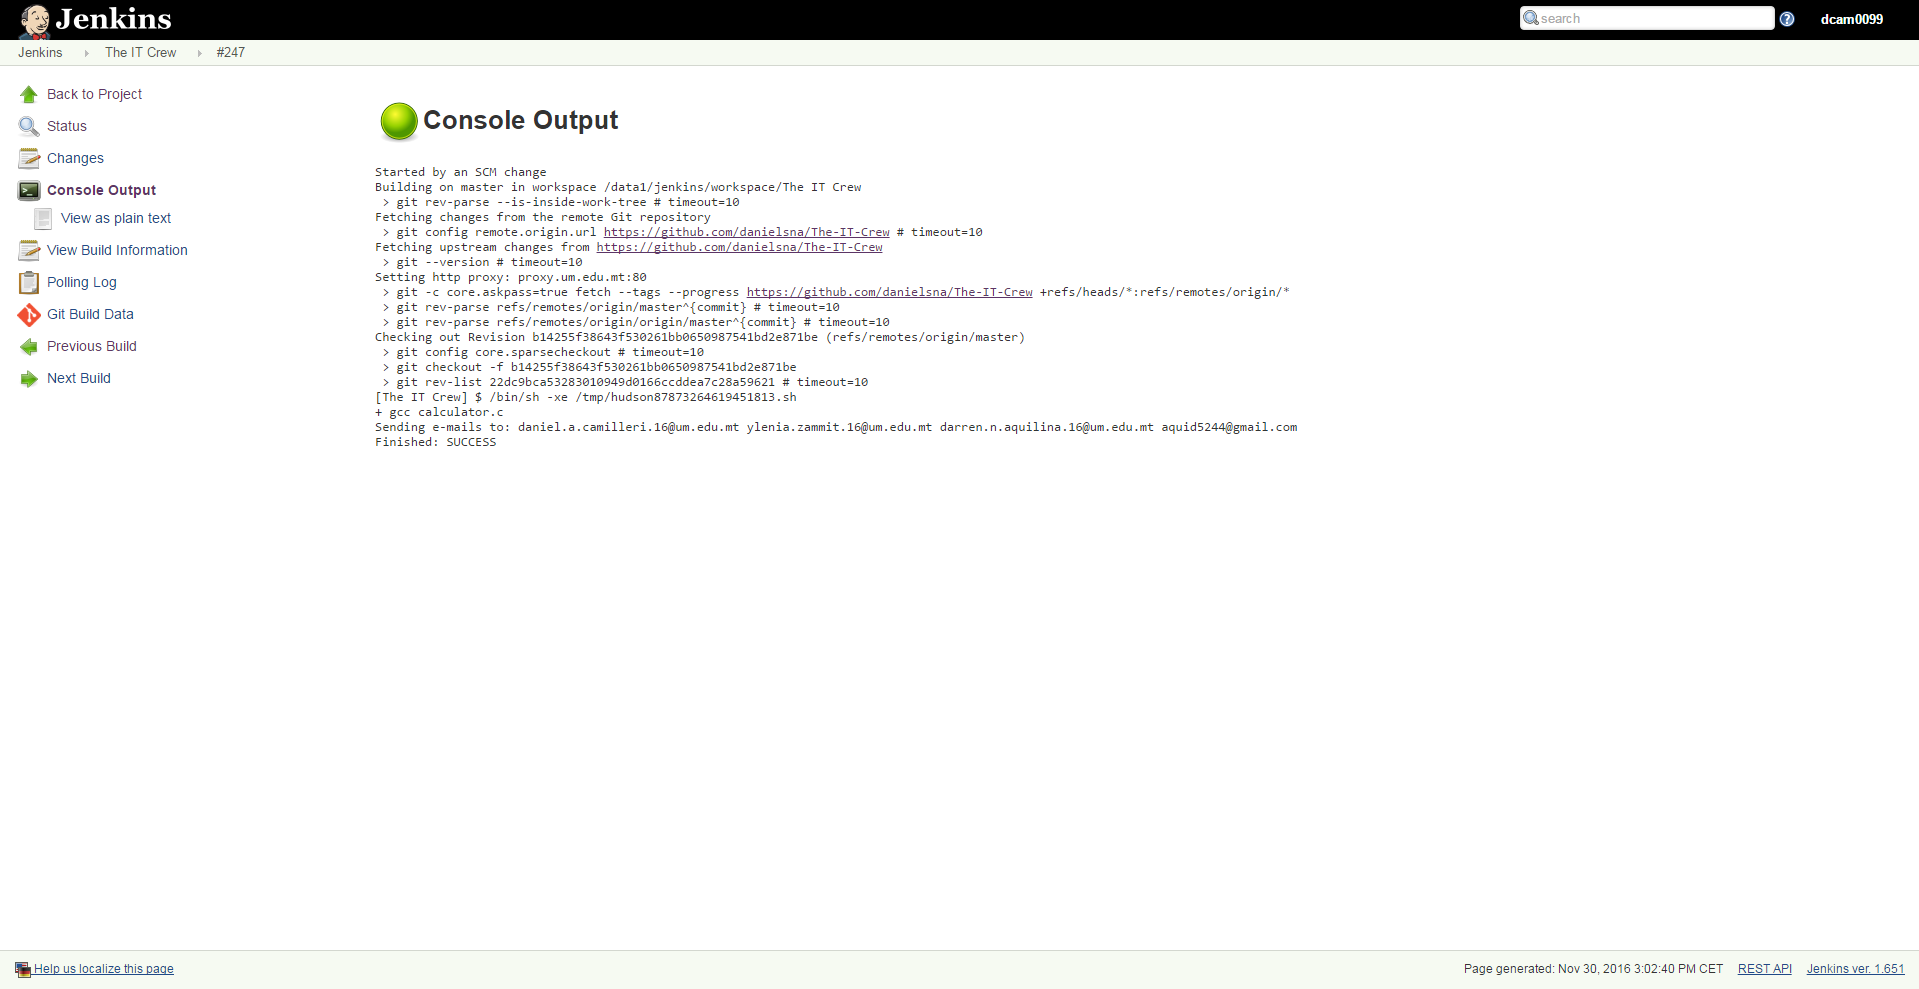
\includegraphics[width=\textwidth, height=\textheight,keepaspectratio]{BreakFix3Darren.PNG}
  \caption{Error fixed by Darren}
\end{figure}

\begin{figure}[h]
  
\includegraphics[width=\textwidth, height=\textheight,keepaspectratio]{Workspace}
  \caption{Error fixed by Darren}
\end{figure}

\newpage
\section{Source Code Listing}
\begin{lstlisting}
calculator.c

#include <stdio.h>
char get_first(void);

int main (void)
{
    char ch;
    float num1, num2;
    num1 = num2 = 0;
    do{
        printf("\nEnter the operation of your choice:
        \na. add\t\ts. 
        subtract\nm.multiply\td. divide\nq.quit");
        ch = get_first();
        switch (ch)
        {
            case 'a':
                printf("\nEnter first number: ");
                while (scanf("%f", &num1) != 1)
                {
                    while (getchar() != '\n');
                    printf("\nPlease enter a number,
                     such as 2.5,
                     -1.78E8, or 3: ");
                }
                printf("\nEnter second number: ");
                while (scanf("%f", &num2) != 1)
                {
                    while (getchar() != '\n');
                    printf("\nPlease enter a number,
                     such as 2.5,
                     -1.78E8, or 3: ");
                }
                printf("%.2f + %.2f = %.2f", num1, num2,
                 num1 + num2);
                while (getchar() != '\n');
                break;
            case 's':
                printf("\nEnter first number: ");
                while (scanf("%f", &num1) != 1)
                {
                    while (getchar() != '\n');
                    printf("\nPlease enter a number,
                     such as 2.5,
                     -1.78E8, or 3: ");
                }
                printf("\nEnter second number: ");
                while (scanf("%f", &num2) != 1)
                {
                    while (getchar() != '\n');
                    printf("\nPlease enter a number,
                     such as 2.5,
                     -1.78E8, or 3: ");
                }
                printf("%.2f - %.2f = %.2f", num1, num2,
                 num1 - num2);
                while (getchar() != '\n');
                break;

            case 'm':
                printf("\nEnter first number: ");
                while (scanf("%f", &num1) != 1)
                {
                    while (getchar() != '\n');
                    printf("\nPlease enter a number,
                     such as 2.5,
                     -1.78E8, or 3: ");
                }
                printf("\nEnter second number: ");
                while (scanf("%f", &num2) != 1)
                {
                    while (getchar() != '\n');
                    printf("\nPlease enter a number,
                     such as 2.5,
                     -1.78E8, or 3: ");
                }
                printf("%.2f * %.2f = %.2f", num1, num2,
                 num1 * num2);
                while (getchar() != '\n');
                break;
            case 'd':

                printf("\nEnter first number: ");
                while (scanf("%f", &num1) != 1)
                {
                    while (getchar() != '\n');
                    printf("\nPlease enter a number,
                     such as 2.5,
                     -1.78E8, or 3: ");
                }

                printf("\nEnter second number: ");
                while ((scanf("%f", &num2) != 1)
                 && num2 == 0)
                {
                    while (getchar() != '\n');
                    printf("\nPlease enter a number
                    other than 0,
                    such as 2.5, -1.78E8, or 3: ");
                }
                printf("%.2f / %.2f = %.2f", num1, num2,
                 num1/num2);
                while (getchar() != '\n');
                break;
            case 'q':
                break;
            default:
                printf("\nPlease enter 'a', 's', 'm', 'd'
                 or 'q' to quit :\n");
        }
    }while (ch != 'q');
    return 0;
}

char get_first(void)

{

    int ch;
    ch = getchar();
    while (getchar() != '\n')
    continue;
	return ch;

}
\end{lstlisting}


\end{document}


